\section{Quantization and Deployment}
\label{sec:quantization}

The deploy stage converts a trained checkpoint into a compact artifact through ternary weight packing \citep{wang_bitnet_2023} and INT8 activation scaling, with size estimates aligned with lightweight deployment goals \citep{samson_lightweight_2026,bravin_embbert_2026}. The same subcommand emits standard or quantized artifacts, or exports HuggingFace Transformers and BitNet GGUF formats for external runtimes. The formulations and size estimates are deferred to Appendix~\ref{sec:annex-norm-bitnet-mod}.

\begin{figure}[t]
\centering
\fitfigure{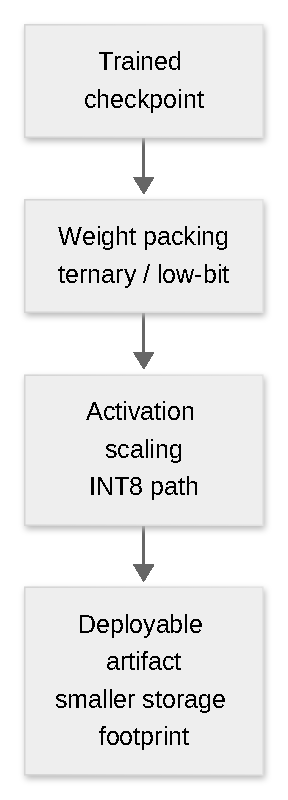
\includegraphics{figures/deploy-flow.pdf}}
\caption{Deployment path from a trained checkpoint to a compact artifact. Quantization is a deploy-stage transformation rather than a separate model family.}
\label{fig:deploy-flow}
\end{figure}
